\section{Semaine 22-23 : 03/07/2023 - 14/07/2023}
\graphicspath{{semaines/semaine_22-23/images/}}

\begin{abstract}
	Je regroupe ici 2 semaines car durant ces 2 dernières semaines, j'ai passé beaucoup de temps sur le rapport dont je n'ai pas encore la date de rendu. Notamment sur la mise en place de la conversion (en python) du rapport latex en un rapport antora et sur la ci permettant de mettre en ligne ce rapport antora à chaque push.
	  
	Après discussion avec Emmanuel, il aimerait que je refasse les mêmes tests sur un carré que ceux effectués sur le cercle. J'ai également essayer de continuer à entraîner avec une loss H1, cette fois sur le carré mais ça ne fonctionne pas. Ces résultats sont obtenus sur les 2 semaines.
\end{abstract}

\subsection{Résultats sur le carré}

On considère ici la solution analytique suivante
$$u_{ex}(x,y)=S\times\sin(2\pi fx+p)\times\sin(2\pi fy+p)$$
avec $S=0.5$, $f=1$ et $p=0$. Solution \textbf{homogène} sur notre domaine, le carré $[0,1]^2$. On prendra $\mathcal{O}=[-0.5,1.5]^2.$

\subsubsection*{Dérivées}

Voici les normes H1 et H2, obtenus avec les différentes méthodes :

\begin{minipage}{\linewidth}
	\centering
	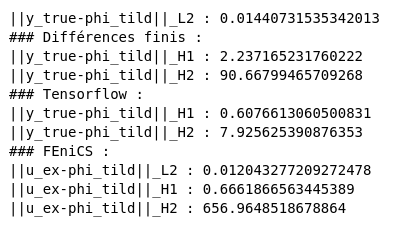
\includegraphics[width=0.4\linewidth]{normes.png}
\end{minipage}

Voici les dérivées premières :

\begin{minipage}{\linewidth}
	\centering
	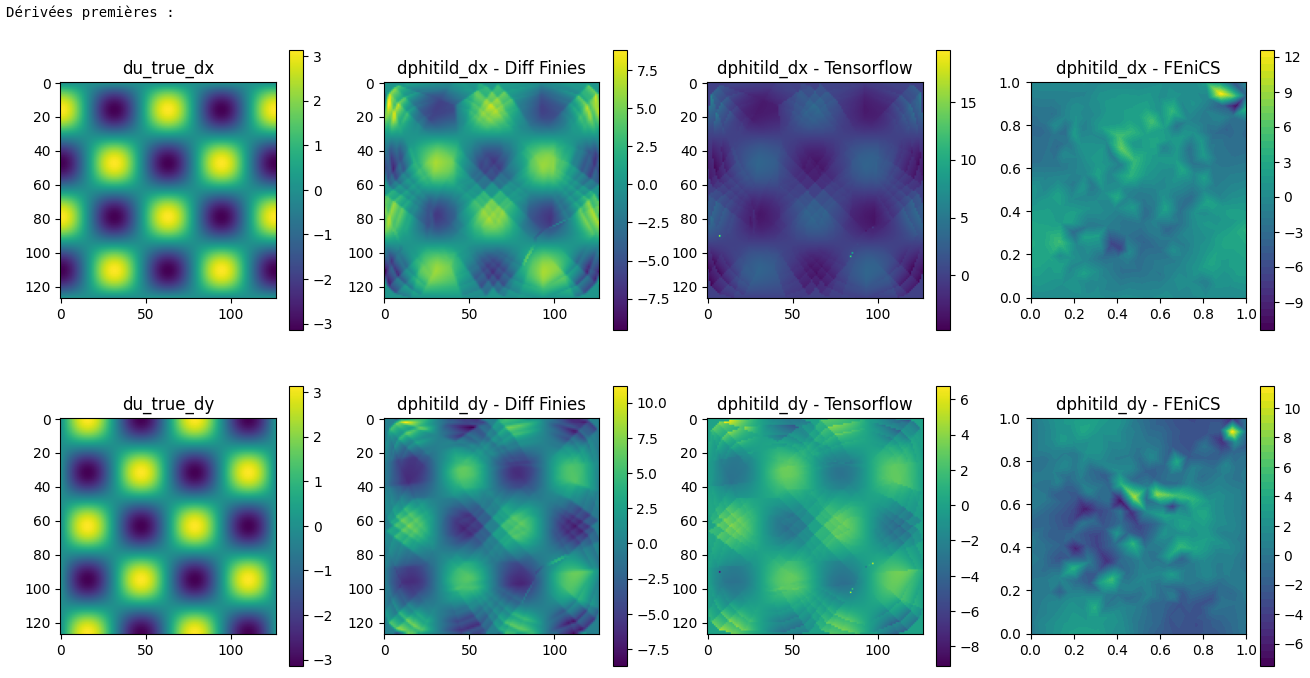
\includegraphics[width=\linewidth]{derivees_premieres.png}
\end{minipage}

\newpage

Voici les dérivées secondes :

\begin{minipage}{\linewidth}
	\centering
	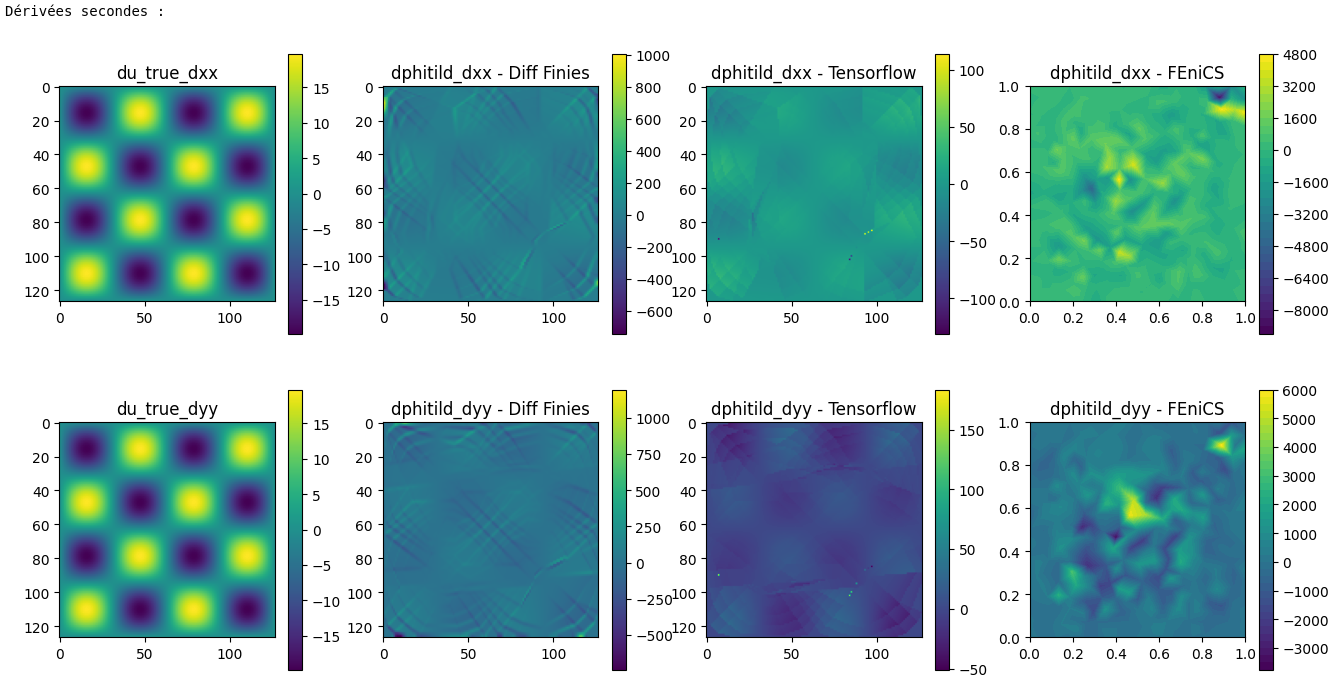
\includegraphics[width=\linewidth]{derivees_secondes.png}
\end{minipage}

\subsubsection*{Comparaison FEM-PhiFEM}

\begin{minipage}{\linewidth}
	\centering
	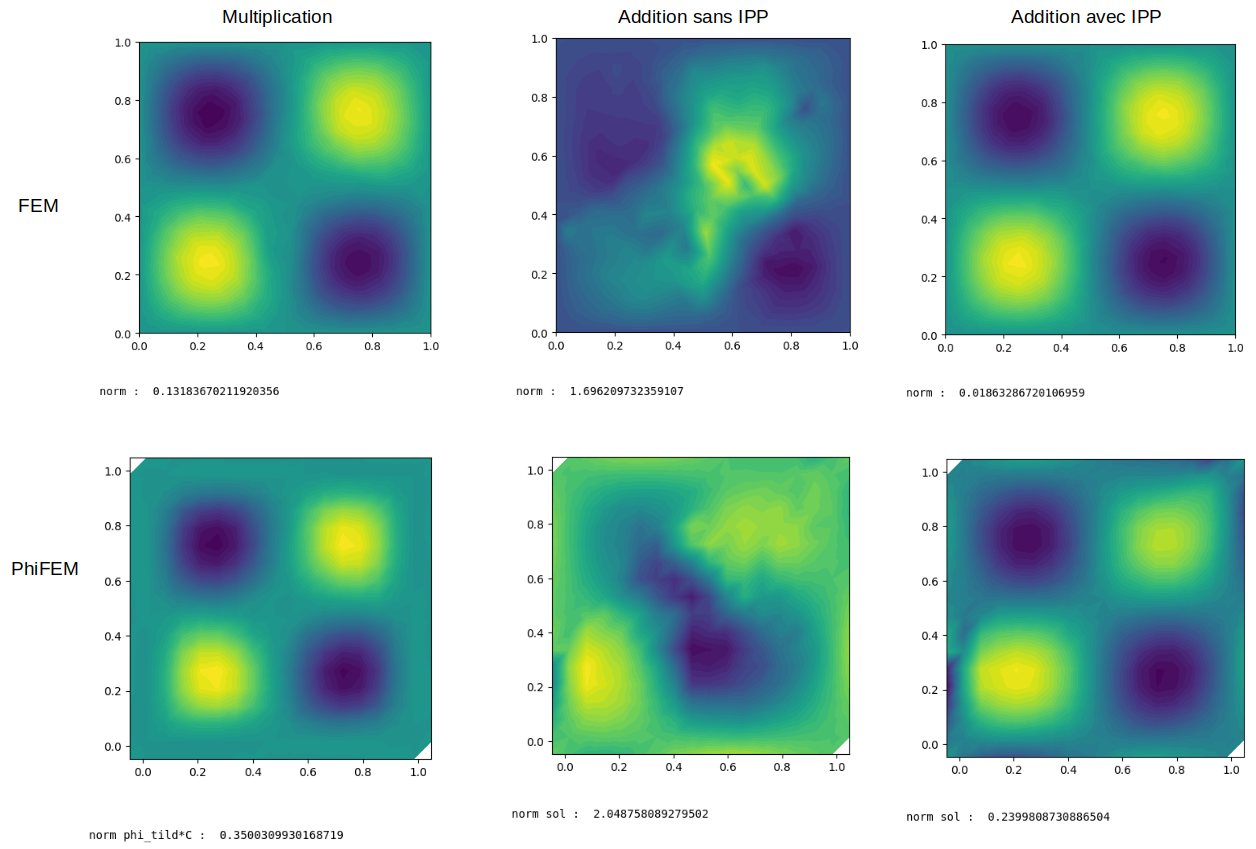
\includegraphics[width=0.9\linewidth]{FEM_vs_PhiFEM.png}
\end{minipage}

\subsection{Entraînement - loss H1}

\begin{minipage}{\linewidth}
	\centering
	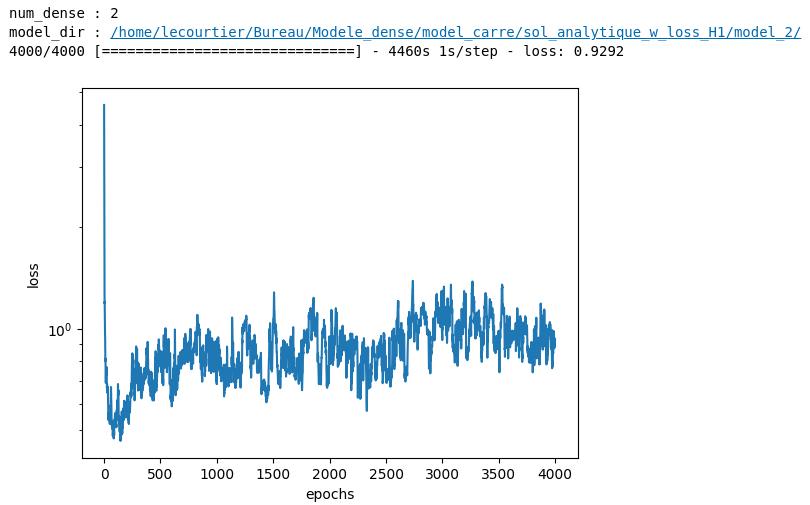
\includegraphics[width=0.6\linewidth]{loss_H1.png}
\end{minipage}

\subsection{Documentation Antora}

\begin{minipage}{\linewidth}
	\centering
	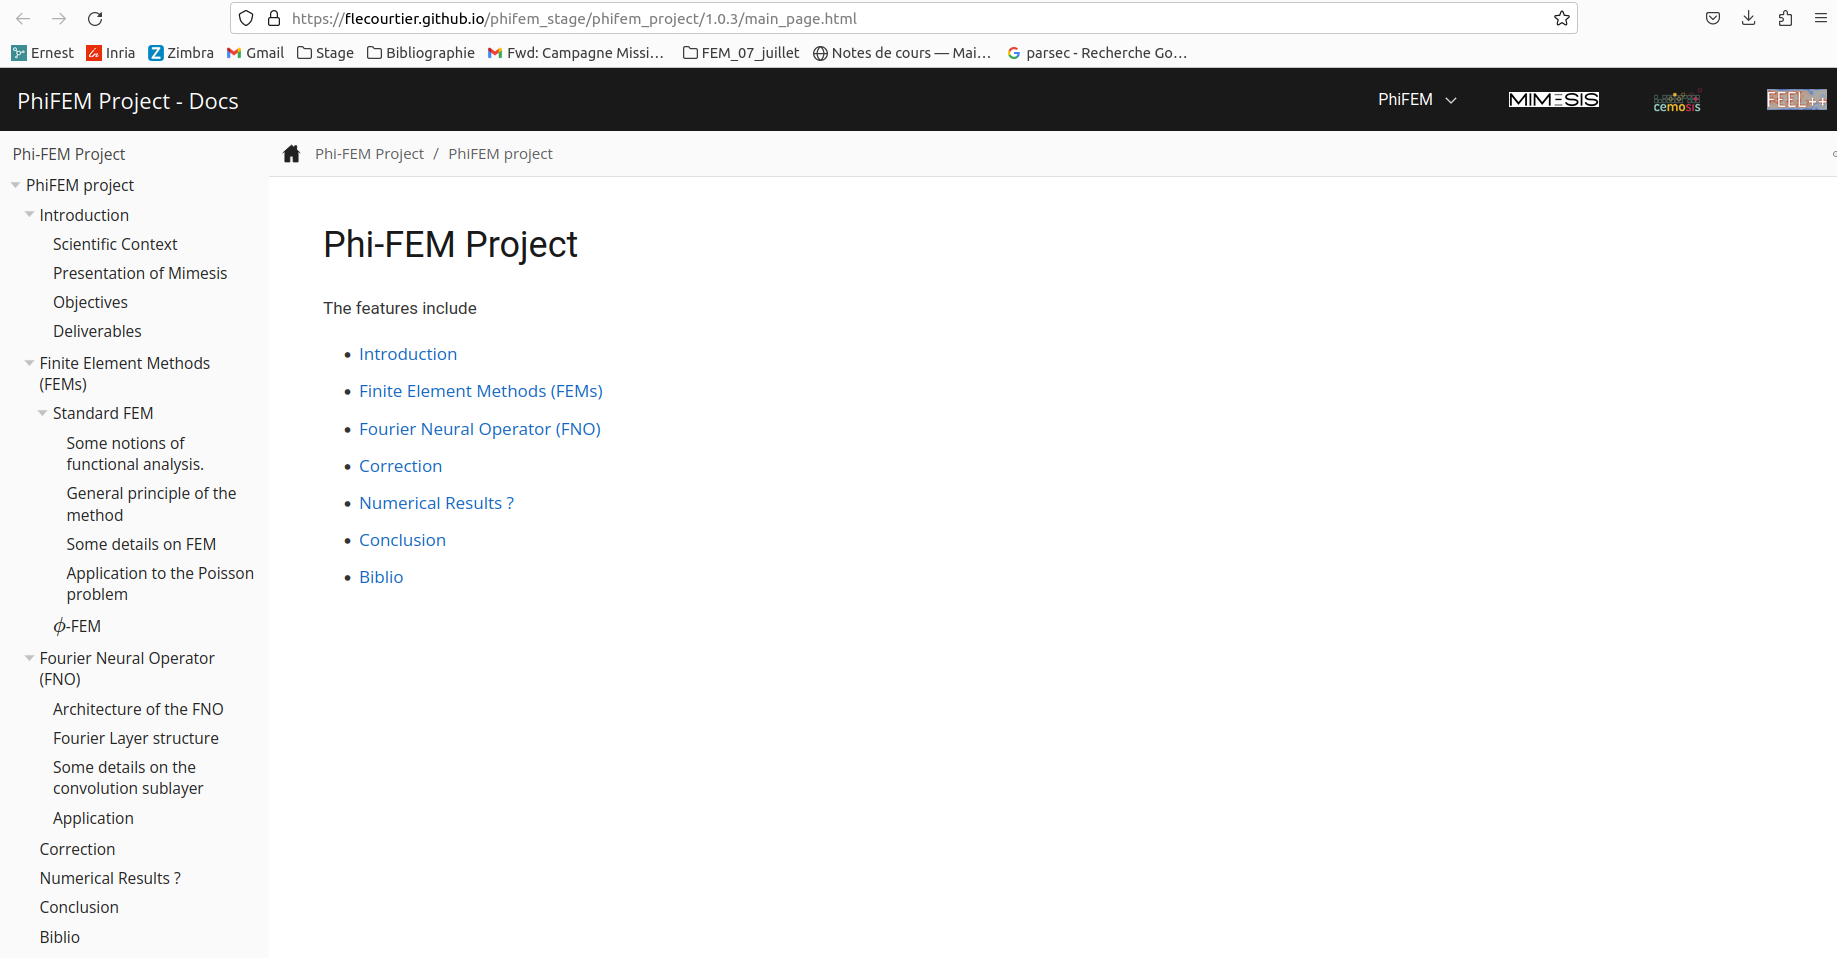
\includegraphics[width=\linewidth]{doc_antora.png}
\end{minipage}

\conclusion{Pour la doc antora, il faut encore faire quelques modifications. Notamment enlever cemosis, FEEL++...}